\section{Background}

In this section, we will delve into the foundational concepts that underpin our discussion in the subsequent sections.

\subsection{eBPF in Kernel}

The Extended Berkeley Packet Filter (eBPF) has blossomed into a multifaceted technology in kernel programming. Evolving from the Berkeley Packet Filter (BPF), eBPF has broadened its horizon from mere packet filtering to a plethora of kernel functionalities, offering a high-performance conduit for user-defined programs to interact within the kernel's privileged domain. Initially tailored for networking tasks, eBPF has now ventured into various kernel subsystems, enabling applications in performance monitoring, security enforcement, and beyond. eBPF operates by allowing pre-compiled programs to be executed within an event-driven framework in response to kernel and userspace events, all under the vigilant scrutiny of a verifier ensuring the kernel's stability and security.

A typical kernel eBPF runtime is depicted in \cref{fig:workflow}. The eBPF program source is compiled using toolchains like clang, and loaded from a userspace eBPF application to the kernel via the BPF syscall, aided by libraries such as libbpf. Post verification, the BPF Just-In-Time (JIT) compiler transmutes the BPF bytecode to machine code for execution. The userspace eBPF application also orchestrates maps to steer the kernel eBPF behavior, aggregate or encapsulate the kernel BPF data, and relay information from the kernel to the user space. Moreover, it can tether BPF programs to events like kprobe, socket, syscall tracepoints, uprobe, and more, furnishing a robust mechanism for real-time interaction and data retrieval.

However, the kernel environment is not without its caveats. Security concerns are paramount -- eBPF programs operate in kernel mode, necessitating root access, which enlarges the attack surface, thereby brewing risks such as container escapes. Inherent vulnerabilities within eBPF could potentially be harnessed for kernel exploits. Furthermore, the verifier curtails the operations of eBPF, and any configuration alteration or enhance demands kernel changes\cite{Zhong22}. Although the community has pondered over unprivileged eBPF, the features it offers in this guise are severely curtailed, lacking the ability to trace syscalls and userspace functions, thus diminishing its appeal.

\begin{figure}[t]
\centering
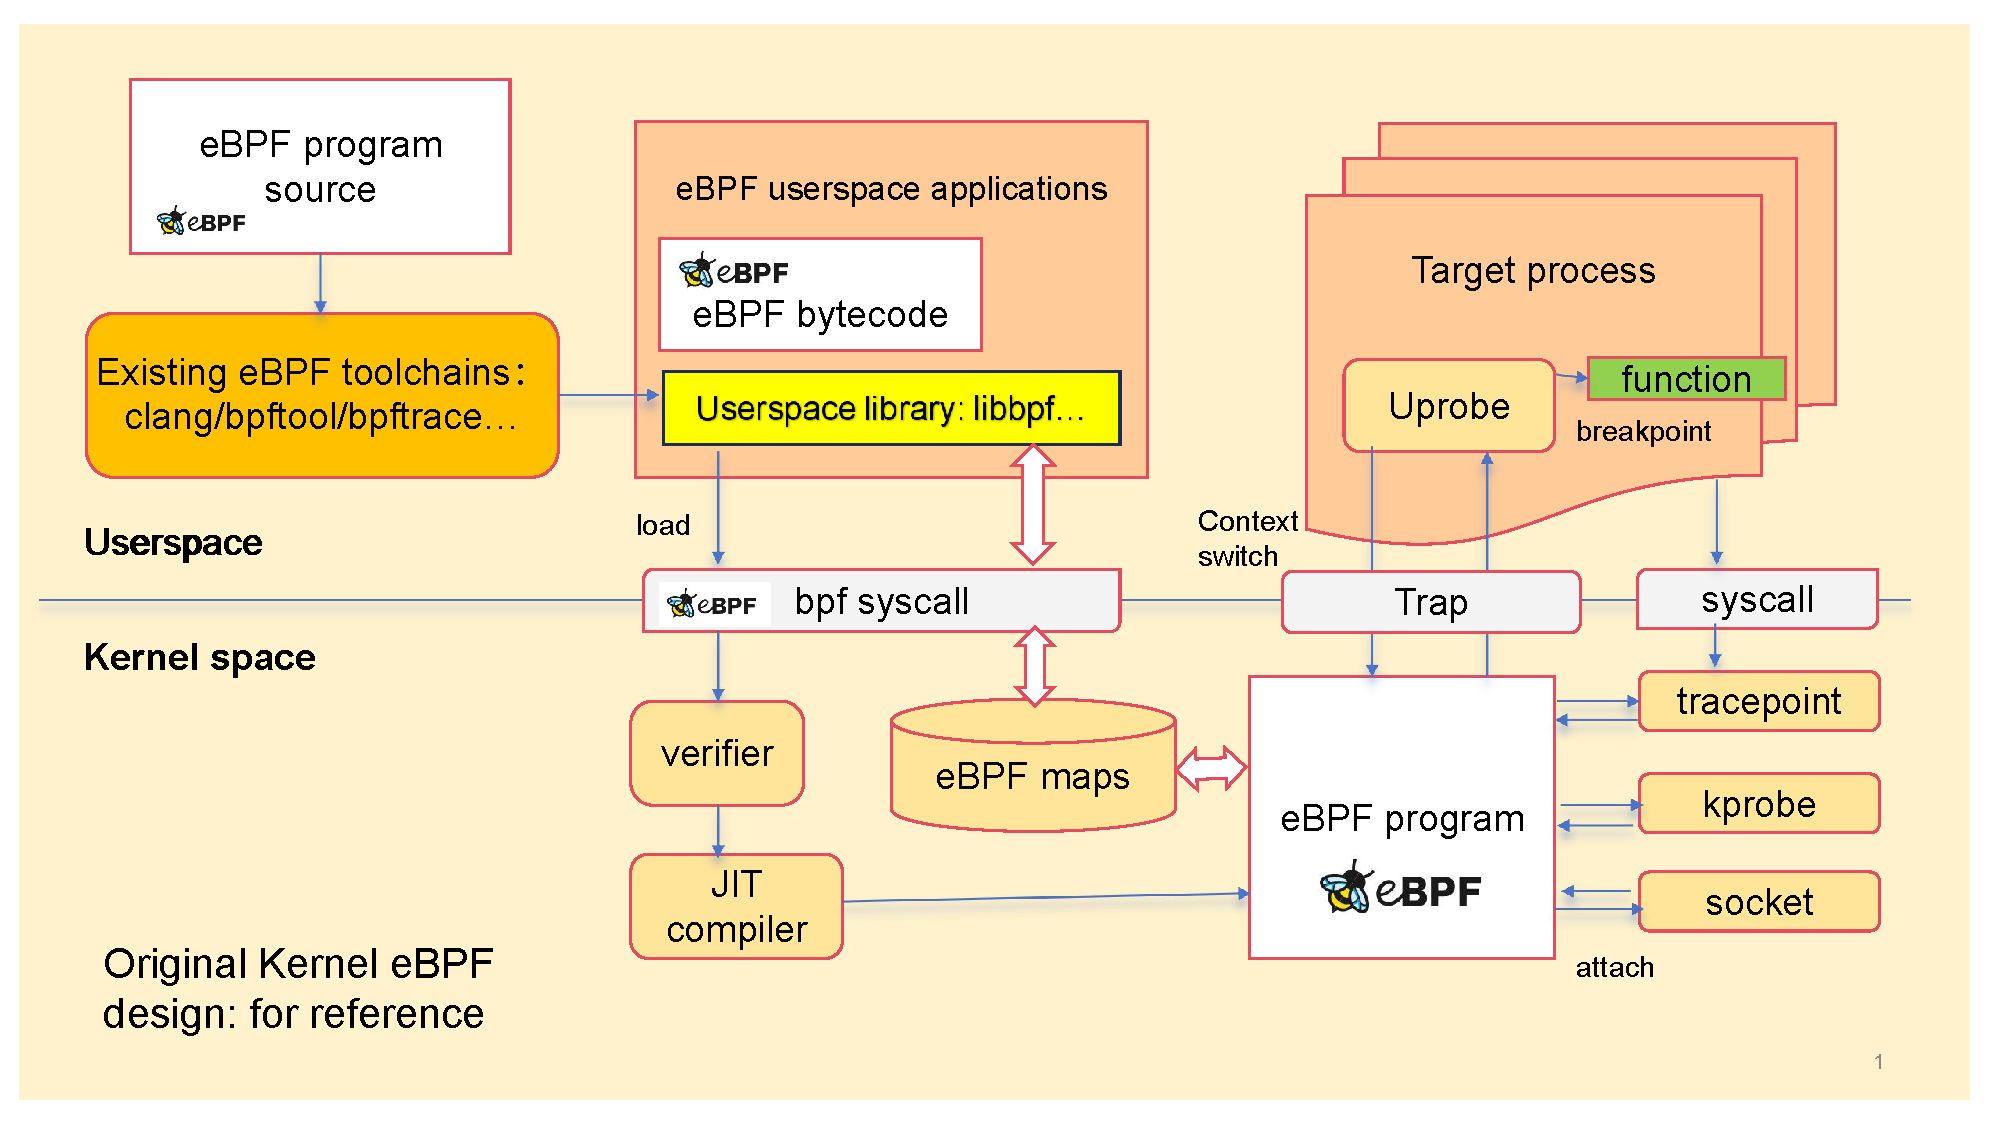
\includegraphics[width=0.5\textwidth]{img/bpftime1.pdf}
\caption{The Workflow of kernel eBPF runtime}\label{fig:workflow}
\end{figure}

\subsection{Uprobe and Syscall Tracepoints}

Uprobes and syscall tracepoints are fundamental mechanisms that enable interaction and introspection within the kernel, particularly when used alongside eBPF. 

\textbf{Uprobes}, which stand for user-level dynamic tracing \cite{keniston2007ptrace}, and are part of perf-tools, allow for dynamic instrumentation of any routine in the user space, facilitating the collection of crucial data for performance analysis and fault diagnosis. Unlike kprobes, which operate within the kernel, uprobes trap into the kernel using the int3 instruction and execute in the kernel space with kernel eBPF, incurring a significant overhead due to the two context switches required - one into the kernel and another back out to the user space. This overhead can often result in a 10 to 20 times slowdown, make it not suitable for real-time monitoring in latency-sensitive applications. Despite the overhead, the combination of uprobes and the eBPF framework provides a powerful tool for non-intrusive tracing of user space functions without necessitating recompilation or restarting user space processes. This has led to its wide adoption in production environments. For instance, uprobes have been utilized for SSL/TLS data capture \cite{ecapture}, memory allocation monitoring and goroutine tracing\cite{bcc} in notable open-source projects. Additionally, they play a significant role in Distributed Tracing Troubleshooting in Zero Code environments, aiding in the identification and resolution of system issues with minimal intrusion into running processes\cite{shen2023network}.

\textbf{Syscall tracepoints} provide a simple way to intercept and modify system calls throughout the system, becoming powerful tools for security and monitoring when used with eBPF. With eBPF, syscall tracepoints can be set up to react to or change system call parameters and return values, allowing detailed control and monitoring of system interactions. In action, when a system call is made, the relevant syscall tracepoint is triggered, starting the connected eBPF program. This eBPF program can inspect the system call parameters, make decisions based on its rules, and even change the return value of the system call. For instance, an eBPF program can be set to block certain system calls by changing the return value to an error code, offering a straightforward way for system call filtering crucial for security. Tracepoints were among the early features brought in with eBPF and have gained wide usage due to their reliability. Unlike kprobes, syscall tracepoints provide a more stable interface and can be used reliably across different kernel versions, making them a favored choice for many. The clear-cut interface of syscall tracepoints reduces the chance of inconsistencies across different kernel versions, establishing the pairing of syscall tracepoints and eBPF as a strong solution for system-wide interception and alteration of system calls.

\subsection{Userspace lightweight isolation: eBPF and Wasm}

The realm of userspace virtual machines has seen the advent of two notable runtimes: eBPF (Extended Berkeley Packet Filter) and Wasm (WebAssembly). Each of these runtimes has distinct design philosophies and operational principles, which cater to varying use-cases and operational requirements.

eBPF, originally rooted in the kernel space, migrated to userspace to alleviate some challenges associated with kernel-based execution. The migration was pioneered by projects like uBPF and rbpf, which aimed to harness the robust capabilities of eBPF while ensuring safer and more convenient user-space operations \cite{ubpf, rbpf}. However, these initial attempts encountered hurdles including the lack of comprehensive support for uprobes and syscalls, the need for manual compilation and program restarts for integration, and an underwhelming hashmap implementation. Despite these limitations, these projects showcased the potential of userspace eBPF runtimes and paved the way for further advancements. For instance, frameworks like RapidPatch and Femto-Containers leveraged eBPF for patch propagation and secure deployment on embedded and IoT devices, demonstrating the versatile applications of eBPF \cite{rapidpatch, femto}. Moreover, projects like DPDK and the ongoing eBPF for Windows initiative indicate substantial progress towards utilizing eBPF benefits across a broader spectrum of applications and platforms \cite{dpdk-ebpf, windows-ebpf}. eBPF prioritizes performance, employing a verifier to ensure security, albeit placing it as a secondary concern.

On the other hand, Wasm is a well-established userspace virtual machine, extensively adopted as a plugin system and a lightweight containerization solution. Its wide language support enables the execution of entire libraries or processes, fostering a rich ecosystem for development. However, Wasm presents some limitations, particularly when it comes to integration. Manual integration is often required, making it less adaptable to API version changes. It relies heavily on underlying libraries for complex operations, such as Wasi-nn, and external APIs like Wasi necessitate additional validation and runtime checks, leading to high performance costs. Unlike eBPF, Wasm emphasizes security, employing Software Fault Isolation (SFI) for security, even at the expense of some runtime overheads.

Both eBPF and Wasm exemplify the strides made in userspace virtual machine technologies, each with its unique strengths and challenges. Their comparative analysis provides a richer understanding of the landscape and the trade-offs involved in leveraging these runtimes for different application domains.